\documentclass[11pt,letterpaper]{article}
\usepackage[T1]{fontenc}
\usepackage[utf8]{inputenc}
\usepackage{lmodern}
\usepackage[margin=0.95in]{geometry}
\usepackage{microtype,amsmath,amssymb,amsthm,mathtools}
\usepackage{booktabs,longtable,tabularx,array,enumitem}
\usepackage{xcolor,graphicx,tikz}
\usetikzlibrary{arrows.meta,positioning,fit}
\usepackage{listings,fancyhdr,xurl,hyperref}
\definecolor{navy}{HTML}{193650}
\definecolor{teal}{HTML}{147D82}
\definecolor{grayink}{HTML}{526272}
\hypersetup{colorlinks=true,linkcolor=navy,urlcolor=teal,citecolor=navy,
  pdftitle={Simplifying the K215 correctness proofs},pdfauthor={Research report prepared for Vladimir Reshetnikov}}
\urlstyle{same}
\pagestyle{fancy}\fancyhf{}
\fancyhead[L]{\small\sffamily K215 / PROOF SIMPLIFICATION}
\fancyhead[R]{\small\sffamily 21 OCTOBER 2026}
\fancyfoot[C]{\small\thepage}
\setlength{\headheight}{14pt}
\setlength{\parskip}{0.35em}
\setlength{\parindent}{0pt}
\setlist{itemsep=0.22em,topsep=0.35em,leftmargin=1.5em}
\renewcommand{\arraystretch}{1.16}
\newcolumntype{Y}{>{\raggedright\arraybackslash}X}
\newcommand{\code}[1]{\texttt{\small\detokenize{#1}}}
\newcommand{\Con}{\operatorname{Con}}
\newcommand{\Halts}{\operatorname{Halts}}
\newcommand{\Reach}{\operatorname{Reach}}
\newcommand{\Valid}{\operatorname{Valid}}
\newcommand{\SemCov}{\operatorname{SemanticCovered}}
\newcommand{\EdgeC}{\operatorname{EdgeContract}}
\newcommand{\PortC}{\operatorname{PortContract}}
\newcommand{\RepoSHA}{2ca3a5c16f0876d2cab842056353c03a1ed2f5f0}
\newcommand{\RepoURL}{https://github.com/VladimirReshetnikov/ProveIt}
\newcommand{\src}[2]{\href{https://github.com/VladimirReshetnikov/ProveIt/blob/2ca3a5c16f0876d2cab842056353c03a1ed2f5f0/#1}{#2}}
\newcommand{\leanfile}[1]{\src{Computability/BusyBeaver/Lean/BusyBeaver/ZFC/#1.lean}{\code{#1.lean}}}
\newcommand{\formalfile}[2]{\src{Computability/BusyBeaver/Research/ZFC/k225-formal/#1}{#2}}
\newtheorem{theorem}{Theorem}[section]
\newtheorem{proposition}[theorem]{Proposition}
\newtheorem{lemma}[theorem]{Lemma}
\theoremstyle{definition}\newtheorem{definition}[theorem]{Definition}
\lstset{basicstyle=\ttfamily\small,columns=fullflexible,breaklines=true,
  keepspaces=true,frame=single,rulecolor=\color{gray!25},backgroundcolor=\color{gray!3},
  xleftmargin=0.5em,xrightmargin=0.5em,aboveskip=0.7em,belowskip=0.7em}
\emergencystretch=2em

\begin{document}
\hypersetup{pageanchor=false}
\begin{titlepage}
\vspace*{0.6in}
{\color{teal}\sffamily\bfseries RESEARCH AND IMPLEMENTATION PROPOSAL\par}
\vspace{0.3in}
{\color{navy}\Huge\bfseries Simplifying the K215\par correctness proofs\par}
\vspace{0.25in}
{\Large Semantic interfaces, smaller imports,\par and shared logical derivations\par}
\vspace{0.4in}
{\large Prepared for Vladimir Reshetnikov\par ProveIt / Busy Beaver / ZFC\par}
\vspace{0.15in}
21 October 2026
\vfill
\begin{minipage}{0.94\textwidth}
\textbf{Main recommendation.} First remove an accidental import of the older
254-state program proof from the K215 semantic calibration. Then make the
register-machine simulation consume semantic block contracts, so a shared
decoder proof and primitive proofs can replace repeated whole-site execution.
A third prototype shares the named-calculus reasoning while retaining the
essential restriction on equality atoms.

\textbf{Measured immediate reduction.} The import patch changes the selected
K215 source closure from 192 to 181 modules, removes a net 198,510 source bytes
and 3,133 source lines, and keeps the old public declarations available.
These are import-closure measurements, not proof-term or timing measurements.

\textbf{Scope.} This packet supplies reviewable patches, mathematical arguments,
targeted Lean checks, and reproducible source measurements. It proposes no
machine-state reduction and makes no new unconditional nonhalting claim.
The canonical 215-state transition table is untouched.
\end{minipage}
\vfill
{\small\color{grayink}Pinned repository snapshot\par
\texttt{\RepoSHA}\par
\href{\RepoURL}{github.com/VladimirReshetnikov/ProveIt}}
\end{titlepage}
\pagenumbering{roman}\hypersetup{pageanchor=true}
\setcounter{tocdepth}{1}
\tableofcontents
\clearpage\pagenumbering{arabic}

\section{What should be simplified next?}

The best next simplification is an architectural one: let each proof layer
state the mathematical behavior it needs, and keep the particular checker that
establishes that behavior behind an adapter. The present repository has already
made substantial progress in this direction. The remaining opportunity is to
complete the separation at two precise boundaries: the import boundary between
set-theoretic semantics and the older 254-state program, and the interface
between site validation and the machine simulation.

This report studies the source at commit \code{2ca3a5c16f}, rather than treating
all earlier research packets as current production code. The latest Lean
implication core has already been reduced to a 58-step condensed-detachment
derivation; shared bundle semantics, normalized source correspondence, shared
Home return, and exact decoder-prefix proofs already exist. Recommending these
again would not answer the next-step question. The repository also contains
older verification receipts and unadopted proposals; their status must be
distinguished from the bytes currently imported by an endpoint.

\begin{table}[ht]
\centering\small
\begin{tabularx}{\textwidth}{@{}p{0.18\textwidth}YY@{}}
\toprule
Priority & Concrete change & What it achieves \\
\midrule
1. Smaller imports & Extract \code{ZFNative.models_ZF}; bypass the unused
\code{WFTheory} import & 192 $\to$ 181 modules in K215's import closure;
old theorem names and legacy modules retained. \\
2. Semantic sites & Add \code{PortContract}, \code{EdgeContract}, and
\code{SemanticCovered}; make the simulation use them & Allows direct
composition of decoder and primitive proofs without re-proving acceptance
by the bounded symbolic executor. \\
3. Shared logic & Factor classical and quantifier reasoning through
\code{NamedDerived}, with explicit equality-atom admissibility & Removes
duplicated proof bodies while preserving the distinction between the
unrestricted and equality-free calculi. \\
4. Rocq alignment & Reconcile the retained Rocq source lane with the
normalized/decode-based checked successor; port the semantic interface &
Uses already available checked work and applies the same architectural
separation to Rocq's stream semantics. \\
\bottomrule
\end{tabularx}
\caption{The proposed order of work. A smaller import closure is an immediate
structural reduction; the semantic interface is the larger subsequent proof-sharing opportunity.}
\end{table}

The second and third changes initially add infrastructure. Their value must not
be reported as a line-count saving before duplicated clients are removed.
In particular, the primitive contracts needed for complete replacement of
\code{KSites215} remain explicit obligations. The packet's verification summary
states exactly which prototypes were compiled and which endpoint builds were
not performed.

\section{The theorem and the existing proof architecture}

\subsection{The exact endpoint}

The Lean endpoint in \leanfile{KEndpoint215} is
\begin{align*}
  \code{BlankHalts machine215}
  &\;\longleftrightarrow\;
  \code{BProv ZFCax_s [] Form.fBot},\\
  \neg\code{BlankHalts machine215}
  &\;\longleftrightarrow\;
  \neg\code{BProv ZFCax_s [] Form.fBot}.
\end{align*}
Thus the right side is the absence of a finite derivation of falsity from the
repository's explicit ZFC axiom predicate. This is the syntactic consistency
statement used by the endpoint. The nonhalting equivalence is obtained from the
halting/refutation equivalence by \code{not_congr}; it should remain that short.

The formal theorem is expressed in Lean's metatheory. The corresponding Rocq
endpoint is expressed in Rocq's metatheory. These facts are distinct from a
separately represented object-language derivation of the equivalence inside ZFC
or PA. The proposals here preserve the existing theorem and its intended
formalization in ZFC; they do not create a new internal arithmetic endpoint.
No step assumes \(\Con(\mathrm{ZFC})\), and no step proves that the machine
actually runs forever without a consistency premise.

The existing Lean endpoint composes the following independent mathematical
claims. The separation is already good and should be retained.

\begin{enumerate}
\item \textbf{Dense/sparse correspondence.} The literal dense machine with
215 working states is a relabeling of the maintained sparse table. The
halting state and blank initial configuration are handled explicitly.
\item \textbf{Bootstrap and tape representation.} The blank machine reaches
the dispatch representation of the empty source path and the chosen register
seed, including the next-candidate value 4.
\item \textbf{Physical simulation.} Every source command is implemented by
one or more concrete Turing-machine transitions, with exact path, gap, and
register behavior.
\item \textbf{Source/enumerator correspondence.} The optimized source and
the command-permuted abstract proof enumerator have equivalent halting behavior.
\item \textbf{Proof-search calibration.} The enumerator halts precisely when
the falsity code is derivable in the compact calculus.
\item \textbf{Logical calibration.} Derivability of that code is equivalent
to a ZF refutation, and the existing constructibility argument transfers
refutability between ZF and ZFC.
\end{enumerate}

The endpoint composition is visible in \leanfile{KEndpoint} and
\leanfile{KEndpoint215}. The other main interfaces are in \leanfile{EnumPerm}
and \leanfile{ConstructibleChoice}. Keeping logical
calibration independent of machine engineering is particularly valuable:
future 215-state variants should reuse it without repeating set theory.

\subsection{What is already present}

The phase-nine report records a 192-module endpoint closure and a 197-module
selected union that also includes five decoder-prefix modules. It records
4,751 site leaves and 6,176 branch outcomes, with the shared Home return already
used by all nine site batches. It reports 984.608 seconds of fresh site
compilation, versus 1,649.340 seconds in the older phase-six records, explicitly
as a historical comparison rather than a paired benchmark.
\formalfile{verification/k215/simplification/phase9/README.md}{[Phase-nine record]}

The latest \leanfile{DominatedImplication} has 295 lines and its
\leanfile{DomRho8} compatibility adapter has 73. The 58-step derivation was
compiled locally in the repository's recorded follow-up; it is later than the
complete phase-nine endpoint check.
\formalfile{rho8cd/PROVEIT_STATUS.md}{[Condensed-detachment status]}

The shared semantics in \leanfile{KSeed222} and \leanfile{KSeedModel222}
already avoid repeating the bundle interpretation in two directions. The
generic decoder entry in \leanfile{KDecoderPrefix215} retains the entire
consumed source word and locates a primitive port uniformly over every gap
and register list. These are foundations for the next change, not proposed
discoveries of this packet.

\subsection{Current-source and receipt comparison}

The source audit in this packet compares hashes rather than inferring current
status from a README. Its results are summarized below. All comparisons are
at the pinned commit, not against a later moving branch.

\begin{center}\small
\begin{tabularx}{\textwidth}{@{}Yrrr@{}}
\toprule
Receipt compared with current source & Match & Differ & Missing \\
\midrule
Lean phase-nine selected union & 196 & 1 & 0 \\
Rocq original local 42-file lane & 41 & 1 & 0 \\
Rocq normalized 44-file successor & 34 & 6 & 4 \\
\bottomrule
\end{tabularx}
\end{center}

The Lean difference is \code{DominatedImplication}, replaced by the later
58-step core. The current Rocq tree largely matches the earlier 42-file local
lane; its differing \code{DomRho8} matches the compact replay in the normalized
receipt. The six differences from the normalized successor are
\code{EnumPerm}, \code{L1_SoundPerm}, \code{L1_CompPerm}, \code{SeedPerm},
\code{L2RootPerm}, and \code{Source215}. The four normalized modules absent
from the current generated lane are \code{PathCodec}, \code{BisimMirror},
\code{NormalizedBisim}, and \code{NormalizedCert215}.

This identifies a retained older Rocq implementation and stale applicability
of some descriptions; it is not evidence that the mathematical equivalence is
false. It does mean that a receipt for one exact source set must not be used as
an exact-source verification claim for another. The reproducible comparison is
included in \code{audit_snapshot.py} and \code{snapshot_audit.json}.

\section{Immediate reduction: separate ZF semantics from the old program}

\subsection{The unnecessary dependency}

The current \leanfile{ZFNative} combines several kinds of result. One of its
theorems, \code{ZFNative.models_ZF}, extracts semantic fields of a ZF model
from satisfaction of the explicit ZF axiom predicate. That theorem does not
refer to an enumerator or a register program. The same file also contains
corollaries about the older program and imports \leanfile{NativeTheory254},
which imports \leanfile{L2Root254}. Consequently a consumer that needs only
the semantic extraction theorem imports the older program proof too.

There are two routes into the K215 endpoint:
\begin{itemize}
\item \leanfile{ConstructibleChoice} imports \code{ZFNative} for its semantic
ZF-model theorem.
\item \leanfile{KQ1ZF} imports \code{WFTheory}, although the relevant
development needs the model interface already supplied by \code{WFModel}.
The stronger \code{WFTheory} imports \code{ZFNative} in turn.
\end{itemize}

This is a dependency problem rather than a hard logical proof. The right
solution is to expose the small semantic interface directly.

\subsection{The four-file patch}

The supplied \code{semantic_import_cut.patch} does exactly the following.
\begin{enumerate}
\item Introduce \code{ZFModelSemantics.lean}, importing only
\code{InternalOrd} and containing the existing theorem
\code{ZFNative.models_ZF} under its original namespace.
\item Make \code{ZFNative.lean} import the new module, and remove the
duplicate original declaration from that file. All remaining legacy
declarations stay available.
\item Change \code{ConstructibleChoice}'s import from \code{ZFNative} to
\code{ZFModelSemantics}.
\item Change \code{KQ1ZF}'s import from \code{WFTheory} to \code{WFModel}.
\end{enumerate}

The moved theorem body is byte-for-byte identical. Its statement is
\[
\begin{split}
 &\bigl(\forall f,\ \mathrm{ZFax\_s}(f)\to\mathrm{Sat}(\mathrm{mem},v,f)\bigr)\\
 &\qquad\Longrightarrow
 \mathrm{ZFAxioms}(\mathrm{mem})\;\land\;
 \bigl(\forall a\,\exists p\,\forall x,
       x\mathrel{\mathrm{mem}}p\leftrightarrow\mathrm{Sub}(\mathrm{mem},x,a)\bigr)
 \;\land\;\mathrm{Regular}(\mathrm{mem}).
\end{split}
\]
The proof simply extracts the finitely named axiom forms and the two schemas,
then applies the existing interpretation lemmas. Moving it does not replace
that argument with an assumption or a new axiom.

\begin{figure}[ht]
\centering
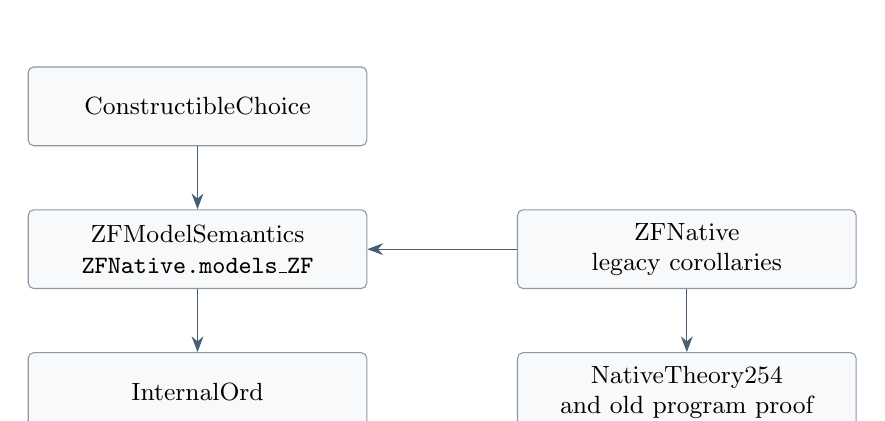
\begin{tikzpicture}[node distance=8mm and 9mm,
 box/.style={draw=navy!50,fill=navy!3,rounded corners=2pt,align=center,
             font=\small,minimum width=43mm,minimum height=10mm},
 arr/.style={-{Stealth[length=2mm]},draw=navy!80}]
\node[box] (cc) {ConstructibleChoice};
\node[box,below=of cc] (sm) {ZFModelSemantics\\\texttt{ZFNative.models\_ZF}};
\node[box,below=of sm] (io) {InternalOrd};
\node[box,right=19mm of sm] (old) {ZFNative\\legacy corollaries};
\node[box,below=of old] (nt) {NativeTheory254\\and old program proof};
\draw[arr] (cc)--(sm); \draw[arr] (sm)--(io);
\draw[arr] (old)--(sm); \draw[arr] (old)--(nt);
\end{tikzpicture}
\caption{The proposed import direction. The semantic consumer no longer
imports the old program; existing clients of \texttt{ZFNative} still do.}
\end{figure}

\subsection{Measured effect and its limits}

The source closure of \code{BusyBeaver.ZFC.KEndpoint215} changes as follows:
\begin{center}
\begin{tabular}{@{}lrrr@{}}
\toprule
Quantity & Before & After & Net reduction \\
\midrule
Project modules & 192 & 181 & 11 \\
Source bytes & 2,363,203 & 2,164,693 & 198,510 \\
Source lines & 45,143 & 42,010 & 3,133 \\
\bottomrule
\end{tabular}
\end{center}

Twelve old modules leave the endpoint's import closure and one new module
enters. The old modules include \code{Dag254}, \code{DecodeFresh254},
\code{L2Lib254}, \code{L2Macros254}, \code{L2Control254},
\code{L2Axioms254}, \code{L2AxiomsEval254}, \code{L2Root254},
\code{NativeDecoded254}, \code{NativeTheory254}, \code{WFTheory}, and
\code{ZFNative}. They remain in the repository for legacy clients.

The resulting reductions are approximately 5.73\% of imported modules,
8.40\% of imported source bytes, and 6.94\% of imported source lines. The
metrics include comments and source data; they are not a theorem-term dependency
analysis. An import can force a module to be compiled even if a final theorem's
proof term never refers to most declarations in that module. Accordingly this
patch simplifies the build and review closure without claiming a corresponding
percentage reduction in logical assumptions, proof-object size, or running time.

The patch is deliberately independent of the machine table, source certificate,
site execution checks, and logical statement. It can be reviewed and adopted
before the larger simulation refactor.

\section{The main architectural proposal: semantic site contracts}

\subsection{Why the current interface blocks reuse}

In \leanfile{KSim}, the current coverage predicate requires, for every input
path, a decoded leaf whose \code{checkEdge} evaluates to \code{true}. That
checker uses a particular symbolic executor, a fixed fuel of 4,000, and a
particular symbolic target representation. Its soundness theorem then supplies
the concrete execution facts needed by the simulation.

A direct proof of a primitive's behavior does not imply that this specific
bounded executor accepts its site. Establishing such acceptance would need a
separate completeness or boundedness argument about the executor, even when
the desired concrete Turing-machine run has already been proved. That extra
obligation serves the implementation of the checker, not the final correctness
theorem.

The proposed change makes the needed concrete execution facts the public
interface. Existing Boolean certificates remain usable through a soundness
adapter. Shared proofs can supply the same interface directly. There is no
assumption that the checker recognizes every correct block.

Earlier decoder-sharing proposals already identified the need for such an
interface. The contribution here is its checked implementation, compatibility
clients, exact connection to the maintained decoder prefix, and a checked
guarded primitive pilot.

\subsection{Precise configurations}

Let \(Q\) be the full consumed source word, \(n\in\mathbb N\) the variable
gap parameter, and \(\vec v\) the physical register list. The current symbolic
dispatch configuration is \code{start Q}; its concrete realization is
\[
 I(Q,n,\vec v)=
 \operatorname{zc}\!\left(84,[1],
 Q\,0^{\,n+(64-|Q|)}\,1\,\operatorname{sepsR}(\vec v)\right).
\]
Here the list operations and natural-number subtraction are exactly those of
\code{conc_start}; the coverage contract requires \(|Q|\le48\). The symbolic
target \code{tgtConf} records the next path, overflow bit, and register-box
effect. Existing lemmas already show how its concrete realization reconstructs
the next representation relation.

For a successful source transition, write \(x\longrightarrow_M^+y\) for
\emph{positive} finite reachability in the physical machine, and
\(x\longrightarrow_M^*y\) for possibly zero transitions. Both conventions
are explicit in the code as \code{Reach1} and \code{Reach}.

\begin{definition}[Run and port contracts]
A \code{RunContract M br source target} is the proposition
\[
 \forall n\,\vec v,
 \ \Valid(\mathrm{br},\vec v)\longrightarrow
 \operatorname{conc}(n,\vec v,\mathrm{source})
 \longrightarrow_M^+
 \operatorname{conc}(n,\vec v,\mathrm{target}).
\]
A \code{PortContract M source Q e} pairs the length and register-index bounds
with the appropriate run contracts for the edge \(e\). A halt edge instead
requires finite reachability to state 230 for every sufficiently long register
list; an internal node edge has contract \(\bot\).
The dispatch specialization is
\[
 \EdgeC_M(Q,e) := \PortC_M(\code{start Q},Q,e).
\]
\end{definition}

For a decrement edge the port contract contains \emph{two} branch-sensitive
proofs. The zero-register branch returns to \code{breakPath 1 Q} without
decrementing; the nonzero branch returns to \code{incPath Q} and decrements
the selected register. A Boolean or propositional test on a concrete small
sample of registers is insufficient: these contracts quantify over arbitrary
register values and gaps.

\subsection{Coverage by semantics}

\begin{definition}[Semantic coverage]
For a register program \(p\), \(\SemCov(M,p)\) asserts
\[
 \begin{split}
 \forall P\ \exists e,d,\quad&
 \mathrm{walk}(p,p.\mathrm{nnodes}+1,p.\mathrm{root},P,0)
       =\mathrm{some}(e,d),\\[-1mm]
 &\EdgeC_M(\mathrm{consume}(P,d),e).
 \end{split}
\]
The consumed word includes the walk's implicit zero padding.
\end{definition}

The patch proves \code{Covered.toSemantic}: the current Boolean coverage
and the usual register-box lemmas imply semantic coverage. It also proves
\code{SemanticCovered.of_leaves}: total source shape plus a semantic contract
for every literal leaf imply semantic coverage. The source-shape check can be
performed independently of symbolic Turing-machine execution.

The existing \code{sim_step}, \code{sim_halt}, and \code{halts_iff} signatures
remain available as compatibility adapters. There is one shared semantic
simulation proof. A small legacy \code{sim_stop} wrapper retains its existing
weaker parameter list; it needs no register-box lemmas.

\begin{theorem}[Simulation from semantic coverage]
Assume \(\SemCov(M,p)\), both actions of terminal state 230 are absent, and
the source configuration \(c\) and physical configuration \(T\) satisfy the
existing representation relation \(\mathrm{Rel}(p,c,T)\). Then
\[
       \Halts_p(c)\quad\longleftrightarrow\quad\Halts_M(T).
\]
\end{theorem}
\begin{proof}
The source walk identifies a leaf and its exact consumed word. The clean-path
invariant rewrites the physical tape into that leaf's dispatch representation.
The semantic contract for the decoded edge supplies positive physical
reachability to the next representation, including the same register update,
or supplies reachability to the terminal state for a halt edge.

For the forward direction, induct on the number of source transitions to the
halt leaf and compose the concrete runs. For the reverse direction, induct
strongly on the length \(t\) of a physical halting run. If the source has
already stopped, coverage excludes a failed decode or internal node, so it is
at its halt leaf. Otherwise the semantic contract produces a positive block
of length \(j+1\). Determinism implies \(j+1\le t\), since a successful
run cannot continue through a halted configuration. The remaining physical
halting run has length \(t-(j+1)<t\), so the induction hypothesis applies.
\end{proof}

This is the mathematical argument already present in \code{KSim}; the patch
changes its input interface rather than introducing a new simulation principle.
No source/physical clock equality is required.

\subsection{Why positive progress must remain}

Replacing \(\longrightarrow^+\) by \(\longrightarrow^*\) in the nonhalting
edge contracts would invalidate the reverse direction. For example, relate a
source state that loops to a physical state that has already halted. Every
source step could then be matched by zero physical steps, while the physical
machine halts and the source does not. The positive-step obligation excludes
this example and makes the induction on the remaining physical time well founded.

A decoder prefix may legitimately have length zero: a primitive could begin
at the initial control position. The \emph{whole successful macro step},
including the primitive and return, must have positive length. This is exactly
the distinction implemented by \code{PortContract.precompose}.

\begin{lemma}[Prefix composition]
Suppose, uniformly in every \(n,\vec v\), the dispatch configuration reaches
a primitive port in zero or more steps. If that port satisfies
\(\PortC_M(\mathrm{port},Q,e)\), then \(\EdgeC_M(Q,e)\).
\end{lemma}
\begin{proof}
For each nonhalting branch, compose the prefix's reflexive-transitive run with
the positive suffix run. For a halt edge, compose the prefix with reachability
to state 230. Bounds on the full word and register index are inherited from
the port contract. This proof treats every branch separately, retaining its
register-validity hypothesis.
\end{proof}

\subsection{Connection to the existing exact decoder prefix}

The current \code{KDecoderPrefix215.leaf_prefix} already gives a uniform
primitive entry. It chooses a decomposition \(Q=\mathrm{pre}\,[b]\), a
physical state \(q\), and a routed source role before quantifying over the
gap and register list. Its target zipper retains
\(\operatorname{reverse}(\mathrm{pre})[1]\) on the left and the unread bit,
gap, marker, and registers on the right.

The new \code{KSemanticSites215} module composes that theorem with an explicit
\code{PrimitiveContracts} premise. It provides the implication
\[
 \mathrm{PrimitiveContracts}
 \;\Longrightarrow\;
 \SemCov(\code{tm215},\code{p215}).
\]
The premise is visible in every resulting theorem; it is not an axiom and is
not claimed to have been established for all primitive families in this packet.
The resulting source/machine equivalence is therefore an integration theorem,
not a replacement completed proof of the full 215-state endpoint.

\section{What can be shared, and what cannot yet be discarded}

\subsection{A reproducible census of primitive obligations}

The exact \code{K215Decoder} source/role arrays give the following census.
The source has 202 nodes and the decoder certificate 234 roles. Its longest
consumed word has 47 bits. The script in the packet parses the literal arrays,
walks the source DAG, counts primitive role entries, and records the pinned input hash.

\begin{center}\small
\begin{tabularx}{\textwidth}{@{}Yrrrr@{}}
\toprule
Operation & Occurrences & Outcomes & Role entries & Role outcomes \\
\midrule
Increment & 1,900 & 1,900 & 32 & 32 \\
Decrement or zero & 1,425 & 2,850 & 38 & 76 \\
Break & 98 & 98 & 7 & 7 \\
Continue & 1,327 & 1,327 & 19 & 19 \\
Halt & 1 & 1 & 1 & 1 \\
\midrule
Total & 4,751 & 6,176 & 97 & 135 \\
\bottomrule
\end{tabularx}
\end{center}

The ratio \(6176/135\approx45.75\) measures potential sharing of role-outcome
families. It is \emph{not} a measured speedup, a proved bound of exactly 135
lemmas, or evidence that all occurrences with a common physical state have the
same tape semantics. Some families may need additional guarded subcases.

\subsection{The continuation is part of the state}

Two source leaves can reach the same physical state and read the same bit yet
have different words to the left of the head. A break or continue instruction
can inspect that prefix, so those entries cannot be identified just by a
physical state number. Similarly, a role's short suffix is insufficient to
recover the full source continuation.

The right grouping key is a \emph{parametric theorem}: the routed role,
operation and branch condition together with a quantified full prefix satisfying
an explicit invariant. The source-to-role certificate establishes that every
occurrence falls under one such theorem. The theorem then implements the
operation for all admissible prefixes, natural gaps and register values.

This is why the proposed interface retains \(Q\) both in the port contract
and in the target path. The exact source walk, its consumed length, and the
primitive's update must all remain connected in the final proof.

\subsection{An incremental replacement strategy}

A practical implementation can maintain a mixture of proof producers. For
each leaf, either an existing Boolean check supplies its semantic contract or
a new family lemma supplies it. There is no need to replace all 4,751 leaves
at once. This supports the following sequence:
\begin{enumerate}
\item Introduce the semantic interface and retain all current site checks.
\item Establish one guarded family at an exact primitive entry; retain its
full prefix and prove the register and gap behavior for all natural values.
\item Prove that every intended occurrence satisfies that family's guard,
using the source/role certificate. Remove only those corresponding old checks.
\item Repeat for decrement branches, break, continue, and the halt case.
\item Once every leaf has a semantic provider, remove the remaining repeated
whole-site execution data and retain the small source-shape check.
\end{enumerate}

The phase-nine packet contains a source-only first CB1 suffix proposal,
associated with 86 literal occurrences and an explicit length guard.
The current packet implements and compiles a successor of that pilot, keeping
the global occurrence-coverage obligation separate. Compiling a suffix theorem
by itself does not prove that all 86 proposed sites satisfy its entry predicate.

\subsection{Checked pilot: the CB1 continuation}

The included \code{KCB1Suffix} and \code{KCB1Contract} modules prove one
concrete family at the semantic interface. Write the consumed word as
\(Q=A001\). At the primitive port the machine is in state 108 reading the
last 1. The three maintained transitions are
\[
 (108,1)\mapsto(0,L,10),\qquad
 (10,0)\mapsto(0,L,16),\qquad
 (16,0)\mapsto(1,L,1).
\]
They rewrite \(A001R\) to \(A100R\), with the head ready to scan the
unchanged prefix \(A\). A finite traversal guard certifies that state 1
returns over \(A\) and the left marker to state 2; the established Home
boundary then returns to the dispatch state 84.

The explicit guard is
\begin{lstlisting}
leftCheck tm215 1 (A.reverse ++ [true]) 2 = true
\end{lstlisting}
and the length premise is \(|A|+3\le48\). The unchanged-word traversal
checker has its own soundness proof. The frame theorem is uniform in an
arbitrary right tape frame \(R\), so no register bound or numerical register
sampling is hidden in this pilot.

The source-path identities are proved separately:
\[
 \operatorname{stripPath}(0,1,A001)=A0,\qquad
 \operatorname{breakPath}(1,A001)=A1,
\]
and the overflow flag is false. The two trailing zero cells become part of the
gap; under the length premise,
\[
 n+\bigl(64-(|A|+3)\bigr)+2
   =n+\bigl(64-(|A|+1)\bigr).
\]
This equality is important because subtraction on natural numbers saturates.
The accepted proof makes the source and target zipper equalities explicit;
the preserved draft's list-association and gap-normalization issues are repaired.

\code{KCB1Contract.port_contract} proves the all-gap, all-register primitive
contract for the actual maintained table. \code{edge_contract} composes it
with \code{leaf_prefix}, assuming the exact source-leaf and routing facts to
state 108 reading true. The remaining task before retiring the 86 proposed
checks is to certify those routing facts and traversal guards for every intended
occurrence. This packet does not claim that finite coverage theorem.

\section{Sharing logical proofs without strengthening the calculus}

\subsection{The repeated mathematical argument}

\leanfile{TarskiDerived} and \leanfile{KThmK} contain parallel named-formula
reasoning: deduction from hypotheses, syllogism, contraposition, double
negation, implication case analysis, quantifier monotonicity, and vacuous
quantification. The two derivability predicates are not identical. In
particular, the restricted calculus must not acquire atomic equality-vacuity
instances just because the unrestricted calculus has them.

A previous structural proposal suggested parameterizing this repeated
development. The \code{NamedDerived} prototype makes that suggestion concrete
while exposing the exact restriction required by the second client.

\subsection{The common interface}

Let \(\mathsf{NF}\) be the existing named-formula type and let
\(D:\mathsf{NF}\to\mathsf{Prop}\) be an arbitrary theorem predicate.
The generic module takes:
\begin{itemize}
\item the existing \code{Kalmar.Classical} interface for implication, falsity,
modus ponens, and the classical propositional basis;
\item four quantifier operations: generalization, distribution of universal
quantification over implication, commutation of quantifiers, and the relevant
\(\exists i\,\forall i\) elimination principle;
\item explicit atomic-vacuity hypotheses, including a predicate specifying
which equality atoms admit them.
\end{itemize}

No numerical formula coding, Cantor pairing, TM state, source program, or
decoder certificate occurs in this interface.

\begin{definition}[Admissible formulas]
For \(E:\mathbb N\to\mathbb N\to\mathsf{Prop}\), define recursively
\[
\begin{array}{rcl}
 \operatorname{Adm}_E(\mathrm{rel}(a,b))&=&\top,\\
 \operatorname{Adm}_E(\mathrm{eq}(a,b))&=&E(a,b),\\
 \operatorname{Adm}_E(\bot)&=&\top,\\
 \operatorname{Adm}_E(A\to B)&=&\operatorname{Adm}_E(A)\land\operatorname{Adm}_E(B),\\
 \operatorname{Adm}_E(\forall j\,A)&=&\operatorname{Adm}_E(A).
\end{array}
\]
\end{definition}

Choosing \(E\equiv\top\) permits all formula atoms. Choosing
\(E\equiv\bot\) restricts to equality-free formulas. The generic theorem
then has the same induction for both clients, while its premises prevent the
restricted client from being silently strengthened.

\begin{theorem}[Guarded vacuous quantification]
Under the common classical and quantifier interfaces and atomic-vacuity
hypotheses, if \(\operatorname{Adm}_E(A)\) and the repository's syntactic
predicate \(\operatorname{Occurs}(i,A)\) is false, then
\[
                   D(A\to\forall i\,A).
\]
\end{theorem}
\begin{proof}
Induct on \(A\). Relation and equality atoms use their respective atomic
hypotheses; the equality case requires the admissibility witness \(E(a,b)\).
Falsity follows from ex falso.

For \(A=B\to C\), the induction hypotheses give vacuous quantification of
\(B\) and \(C\). The common quantifier rules derive vacuous quantification
of \(\neg B\). Universal monotonicity then gives
\(\neg B\to\forall i(B\to C)\) and
\(C\to\forall i(B\to C)\). The shared classical implication case lemma
combines these into \((B\to C)\to\forall i(B\to C)\).

For \(A=\forall j\,B\), apply universal monotonicity at \(j\) to the
induction hypothesis and then commute the quantifiers. Each use of nonoccurrence
is the same syntactic premise as in the original theorem, not an informal
substitution of ``not free'' for a stronger existing condition.
\end{proof}

\subsection{Compatibility and honest size accounting}

The original theorem namespaces and statement shapes are retained as adapters.
The packet includes a client that instantiates the original interfaces of both
calculi and prints axiom reports for the generic and specialized vacuity
theorems. A downstream \code{KEind222} check exercises the restricted-calculus
consumer, rather than only compiling a standalone abstract lemma.

The first explicit-signature implementation grows the combined source rather
than shrinking it. This is expected when two clients retain named public
wrappers and a third file adds the common interface. The appropriate claim is
one proof of the repeated reasoning and two checked specializations.
The final compact-alias implementation has the following accounting:
\begin{center}\small
\begin{tabular}{@{}lrr@{}}
\toprule
Production file & Original lines & Proposed lines \\
\midrule
\code{TarskiDerived} & 183 & 136 \\
\code{KThmK} & 320 & 295 \\
\code{NamedDerived} & 0 & 168 \\
\midrule
Combined & 503 & 599 \\
\bottomrule
\end{tabular}
\end{center}
The byte count grows from 21,694 to 23,660. Thirty-eight public derived-rule
bodies become type-compatible transparent aliases; the two vacuity declarations
remain theorems. This is a checked maintenance prototype, with an initial cost
of 96 lines and 1,966 bytes, rather than the report's headline reduction.
If physical source length is the overriding objective, adopt the import cut
first and defer this factorization; flattening carefully named lemmas merely
to save wrapper lines can make proof terms and maintenance worse.

\section{Applying the same approach to Rocq}

\subsection{Use the actual retained source lane}

The current Rocq lane has not adopted every change described in the later
normalized receipt. The shortest immediate route is to reconcile and replay
that existing checked successor, rather than independently rediscover the
same normalization and command-level decomposition. Both maintained templates
and generated files must be updated together. An edit only to
\code{coq/215/Source215.v} is not a durable refactor if regeneration restores
the older template.

The relevant existing improvements are a normalized source certificate with
one correspondence and symmetry, command decoding followed by a small
\code{xstep}, and a completeness interface valid from an arbitrary candidate
boundary. The older seed file visibly duplicates a reachability induction;
the normalized/decode-based successor already removes that duplication.
The repository's earlier one-rank scheduler proposal can be evaluated separately
if arbitrary initial proof-list pointers are desired. It is not new work in
this packet.

\subsection{The semantic boundary in the stream-based simulator}

The concrete port is visible in
\formalfile{rocq/rocq-extension/coq/215/Sim230.v}{\code{Sim230.v}}.
Its \code{inv_view} returns a successful \code{check_edge} equation;
\code{inv_step} unpacks that Boolean result and calls \code{site_run'}, while
\code{inv_halt} uses \code{site_halt'}. The proof then consumes only positive
reachability and terminal behavior.

The Rocq adaptation should therefore introduce a proposition \code{edge_spec}
whose cases state the concrete branch-sensitive runs, length and register-index
bounds, and terminal reachability. Prove
\[
       \code{check_edge Q e = true}\ \Longrightarrow\ \code{edge_spec Q e}
\]
from the existing checker-soundness theorems. Have \code{inv_view} expose
\code{edge_spec} and have \code{inv_step}/\code{inv_halt} consume it directly.
The existing proof of \code{tm230_rm} in
\formalfile{rocq/rocq-extension/coq/215/Sim230Main.v}{\code{Sim230Main.v}}
continues to use the same progress argument.

This port should use Rocq's own tape and progress relations. Replacing its
stream semantics by Lean's zipper representation would create a second
unnecessary correspondence theorem. Share the mathematical contract and the
finite source/role data; let each prover retain its native representation and
kernel-checked implementation.

\subsection{What should be shared across provers}

The most stable common artifacts are small, representation-neutral data:
source/role graphs, normalized correspondence pairs, primitive operation tags,
register permutations, and condensed-detachment dependency edges. Python can
generate these aggressively because its output is checked by each kernel.
The generator must not become an axiom about correctness.

The semantic proof should be written once per prover over an abstract
interface. This is a much smaller duplication than re-proving each machine
variant and each source occurrence. It also preserves useful independence:
Rocq and Lean need not share tactic scripts or trusted evaluation mechanisms.

The current packet does not claim a new Rocq kernel run for the proposed
semantic-site refactor. Its Rocq section is a precise port plan grounded in
the actual current \code{Sim230} proof, while the implementation pilot and
new compilation receipts are in Lean.

\section{Validation, trust, and reproducibility}

\subsection{What the targeted checks establish}

The packet uses Lean 4.32.0, the toolchain named by the repository. Each
selected module is compiled into a fresh task-specific object directory, using
the pinned source plus an explicit overlay. Unchanged objects can be reused
only when the compiler identity, module bytes, direct imports, transitive
source fingerprints, and output hashes agree.

This last requirement is material. A changed executable definition may affect
kernel reduction in downstream \code{decide} proofs even if an intermediate
compiled object happens to be byte-identical. The phase-nine history already
records this failure mode. The supplied targeted driver keys reuse by the
entire transitive source/import fingerprint, not just immediate object hashes.

The compact verification summary accompanies the raw per-module logs and
source-hash ledger. A successful targeted build checks the included new
theorem bodies and named compatibility clients. It is not a second full replay
of the 215-state endpoint or the entire Rocq closure.

\begin{center}\small
\begin{tabularx}{\textwidth}{@{}p{0.22\textwidth}rY@{}}
\toprule
Accepted check & Modules & Checked scope \\
\midrule
Import cut & 123 & 99 freshly compiled, 24 matched providers reused;
generic endpoint, semantic ancestors, original legacy facade and eight
named assumption reports. \\
Semantic sites & 27 & Final source closure of \code{KSimCompatibility},
\code{KSemanticSites215}, and \code{KCB1Contract}; accepted providers and
their original logs retained. \\
Shared named logic & 16 & 13 freshly compiled, 3 matched providers reused;
both old interfaces and the actual \code{KEind222} consumer. \\
\bottomrule
\end{tabularx}
\end{center}

The import-cut audit has no warnings; its inherited source ancestry retains
twelve linter warnings in seven unchanged modules. The accepted new machine
clients have no warnings. The complete machine-specific \code{KEndpoint215}
closure was not rebuilt in this packet, and no new Rocq compilation is claimed.
The three proposal checks are separate checks of their respective overlays;
they do not assert that a combined production checkpoint has been replayed.

The \code{KSim} interface change itself grows that module from 356 to 506
lines. Its five supplied source modules, including audit and pilot clients,
total 778 lines. Fifteen original executable/interface definitions are
byte-identical, including \code{checkEdge}, \code{start}, \code{tgtConf},
\code{Covered}, and \code{Rel}. The subsequent removal of repeated leaf
checks is where a net machine-layer source reduction can be measured.

\subsection{Acceptance checks for each change}

For the import cut, the essential checks are: the moved theorem has its original
type and body; old \code{ZFNative} clients still compile; the changed semantic
consumers and generic endpoint compile; and the static import graph actually
loses the twelve unwanted modules. There is no reason to recompute every
physical site merely to validate those import edits.

For the semantic interface, check the old public \code{KSim} theorem types,
the new semantic equivalence, the Boolean adapter, and the decoder-prefix
composition. The first primitive-family pilot must quantify over arbitrary
registers and gaps and retain every guard. A later replacement of actual site
providers does require checking all changed source-dependent descendants and
the concrete endpoint client.

For shared logic, check both specializations, a downstream restricted-calculus
consumer, and the axiom reports. The type of the generic theorem must include
the equality-atom admissibility premise; a proof of a stronger unrestricted
calculus would not be an acceptable substitute.

\subsection{Axiom reports and limitations}

The repository's recorded closed Lean endpoint audits use
\code{propext}, \code{Classical.choice}, and \code{Quot.sound}. The targeted
prototype reports are listed in the delivered verification summary. An
explicit theorem argument such as \code{PrimitiveContracts} is a hypothesis,
not a newly asserted global axiom; it must still be discharged before the
semantic route becomes a closed machine endpoint.

The moved \code{models_ZF} theorem and new \code{Semantic.halts_iff} use
\code{propext} and \code{Quot.sound}. The source-shape check has no axioms.
The CB1 port contract uses \code{propext} and \code{Quot.sound}; its composed
edge contract additionally uses \code{Classical.choice} through the existing
decoder prefix. The generic and specialized vacuity theorems report only
\code{propext}. The original restricted specialization and alpha-renaming
theorems retain their existing three standard axioms. No \code{sorry} or new
postulate is introduced by the accepted prototypes.

No timing improvement is inferred from source measurements. No lower bound on
machine size is inferred from a failed simplification. No claim that 135 role
outcomes have all been proved follows from counting them. These distinctions
make the packet usable as a concrete next development step rather than an
overstated new correctness certificate.

\section{Recommended implementation sequence}

\begin{enumerate}
\item \textbf{Adopt the semantic import cut.} It is the smallest patch, moves
one existing theorem verbatim, and immediately removes the obsolete program
layer from K215's imported source closure. Keep legacy facades and public names.
\item \textbf{Adopt the semantic \code{KSim} interface with old checks intact.}
This creates an independently checkable compatibility checkpoint. The machine
table and current leaf certificates need no alteration at this stage.
\item \textbf{Complete one exact primitive family.} Use the established
decoder port, the existing register-box contracts, and the shared Home return.
Prove the full continuation law and then certify which source leaves instantiate
it. Replace only those leaf checks.
\item \textbf{Scale by operation families.} Decrement has the largest outcome
count and requires separate zero/nonzero branches. Break and continue need
especially careful full-prefix invariants. Halt has its own terminal contract.
\item \textbf{Factor logical derivations if maintenance is the objective.}
The generic \code{NamedDerived} proof removes duplicated reasoning but its
compatibility wrappers initially increase source length. Keep that tradeoff
explicit in review.
\item \textbf{Bring the Rocq lane to the chosen checkpoint.} Reuse the already
checked normalized successor where appropriate, synchronize generators, and
apply the same semantic interface over Rocq's existing relations. Then perform
the maintained recursive kernel audit for the selected final source set.
\end{enumerate}

The most valuable long-term shape is a short composition theorem whose inputs
are independently named semantic contracts. The expensive work then lives in
small reusable lemmas and finite certificates, with clear ownership of the
source word, continuation, register effect, and positive physical progress.

\appendix
\section{Packet contents and use}

The archive contains the \LaTeX{} source and compiled PDF of this report,
separate overlays and patches for the proposed changes, audit clients,
reproduction scripts, source measurements, and compilation receipts. It omits
compiler binaries and compiled proof objects. \code{README.md} gives the exact
layout and the final verification scope.

To review a patch against the pinned checkout, use \code{git apply --check}
first. The overlays are alternatives to applying patches: the supplied
\code{scripts/check_lean.py} resolves an explicit overlay before the four
project source roots, builds only the requested import closure, and records its
source and compiler identity. Its output directory should be separate for each
proposal. The patch sets are separated so the small import change can be
adopted independently of the larger simulation and logical refactors.

The repository's full endpoint build commands remain the appropriate final
gate when a combined production checkpoint is selected. The packet's targeted
checks are designed to avoid unnecessary repeats of expensive unchanged
site checks while establishing that the proposed interfaces elaborate.

\section{Source guide}

All links below point to the pinned commit. The companion measurement JSON
files provide the exact paths and hashes used by this report.
\begin{enumerate}
\item \leanfile{KEndpoint215} and \leanfile{KEndpoint}: literal-machine endpoint
and generic composition.
\item \leanfile{ZFNative}, \leanfile{NativeTheory254},
\leanfile{ConstructibleChoice}, and \leanfile{KQ1ZF}: the semantic import cut.
\item \leanfile{KSim}: current Boolean coverage, physical representation,
and the two-direction halting simulation.
\item \leanfile{KDecoderPrefix215}, \leanfile{K215Decoder}, and
\leanfile{DecoderSourceBinding}: exact primitive entry and source/role binding.
\item \leanfile{KSites215}: current leaf coverage assembled from nine batches.
\item \leanfile{TarskiDerived}, \leanfile{KThmK}, and
\leanfile{TarskiCalculus}: the shared named-calculus prototype.
\item \formalfile{verification/k215/simplification/phase9/README.md}{Phase-nine
summary}, \formalfile{verification/k215/lean/README.md}{Lean endpoint-check
instructions}, and \formalfile{rho8cd/PROVEIT_STATUS.md}{latest implication-core
status}: historical and current verification boundaries.
\item \formalfile{verification/k215/rocq/normalized-91/README.md}{Normalized
Rocq receipt} and \formalfile{rocq/rocq-extension/coq/215/Sim230.v}{current
Rocq simulation}: distinct source checkpoints used in the comparison.
\end{enumerate}

\section{Attribution}

The underlying compact theory, proof enumerator, register compiler, Turing
machine, and existing formal proofs belong to the ProveIt project and the
contributors credited in its preserved notices, including Elliot Glazer,
Jeff Ketchersid, Andrew James Wade, BusyCoq, and the Coq Library of
Undecidability within their respective scopes. This packet refactors and extends
that work. It does not claim priority for the existing normalized certificate,
condensed-detachment proof, exact decoder prefix, shared Home return, or the
earlier proposal to parameterize the named-calculus derivations.

The original source headers are retained in modified files. The supplied
attribution notice points to the repository's inherited terms. Repository
material is not relicensed merely by inclusion in a research packet.

\end{document}
